\documentclass[12pt,letterpaper]{article}
\usepackage[latin1]{inputenc}
\usepackage{amsmath}
\usepackage{amsfonts}
\usepackage{amssymb}
\usepackage{amsthm}
\usepackage{enumerate}
\usepackage[margin=1in]{geometry}
\usepackage{graphicx}

\newtheorem{theorem}{Theorem}[section]
\newtheorem{rem}[theorem]{Remark}
\newenvironment{remark}{\begin{rem}\rm}{\end{rem}}
\newtheorem{claim}[theorem]{Claim}
\newtheorem{lemma}[theorem]{Lemma}
\newtheorem{proposition}[theorem]{Proposition}
\newtheorem{corollary}[theorem]{Corollary}
\newtheorem{eg}[theorem]{Example}
\newenvironment{example}{\begin{eg}\rm}{\end{eg}}
\newtheorem{definition}[theorem]{Definition}

\newcommand{\C}{\mathbb{C}}
\newcommand{\R}{\mathbb{R}}
\newcommand{\abs}[1]{\lvert#1\rvert}
\newcommand{\len}[1]{\lVert#1\rVert}
\newcommand{\di}{\displaystyle}
\DeclareMathOperator{\Real}{Re}
\DeclareMathOperator{\Img}{Im}
\newcommand{\x}{\mathbf{x}}
\newcommand{\y}{\mathbf{y}}
\newcommand{\dotp}{\boldsymbol{\cdot}}
\author{Sean Fitzpatrick}
\title{Some Basic Topology in $\R^n$}

\begin{document}
\maketitle
\begin{abstract}
This is a quick summary of some of the ideas from topology that are essential to the study of functions of several variables. We'll avoid any discussion of topology in a general sense and stick to open sets, limits, etc. as they are described in $\R^n$ using the standard distance formula.
\end{abstract}
\section{Distances as lengths of vectors}
Recall that the {\em length} (magnitude) of a vector $\x = \langle x_1, x_2, \ldots,x_n\rangle \in\R^n$ is given by
\begin{equation}\label{mod}
\lVert\x\rVert = \sqrt{x_1^2+x_2^2+\cdots+ x_n^2}.
\end{equation}
In the following pages, we will describe the properties of the length function, and explain how it equips $\R^n$ with the structure needed to define limits and continuity (and thence, derivatives and integrals of functions of a several variables).  
\begin{proposition}\label{prop1}
The length $\lVert\x\rVert$ of a vector $\x\in\R^n$, as defined by \eqref{mod}, satisfies the following properties, the proof of which we leave to the reader:
\begin{enumerate}[(i)]
\item $\len{c\x} = \abs{c}\len{\x}$ for all $\x\in\R^n$ and $c\in\R$.
\item $\len{\x+\y} \leq \len{\x}+\len{\y}$ for all $\x,\y\in\R^n$.
\item $\len{\x-\y} \geq \left|\len{\x}-\len{\y}\right|$ for all $\x,\y\in \R^n$.
\item $\abs{\x\dotp\y} = \abs{x_1y_1+\cdots + x_ny_n}\leq \len{\x}\len{\y}$ for all $\x,\y\in\R^n$ (the Cauchy-Schwarz inequality).
\end{enumerate}
\end{proposition}
\begin{center}
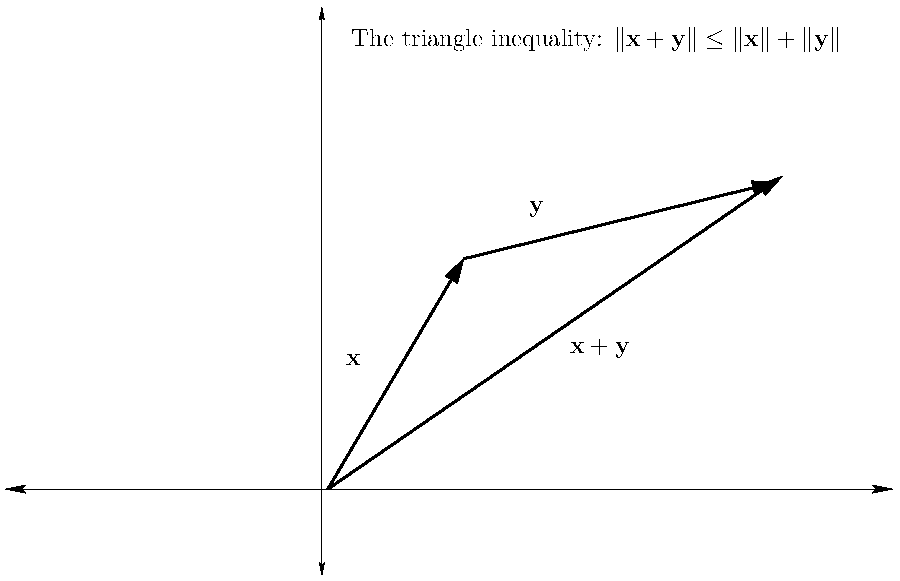
\includegraphics[width=5in]{triangle.pdf}
\end{center}
Having established the above properties of the length of a vector, we use it to define a {\em distance function} between points in $\R^n$. Let $\x$ and $\y$ be the position vectors corresponding to points $P(x_1,\ldots, x_n)$ and $Q(y_1,\ldots, y_n)$, respectively. We define the distance between $P$ and $Q$ by \begin{equation}\label{dist}
d(P,Q)=\len{\x-\y}.
\end{equation}
It follows from \eqref{mod} and the above proposition that $d(P,Q)$ satisfies the following (exercise):
\begin{proposition}
For any points $P,Q\in \R^n$, we have:
\begin{enumerate}[(a)]
\item $d(P,Q)\geq 0$, and $d(P,Q)=0$ if and only if $P=Q$.
\item $d(P,Q)=d(Q,P)$.
\item $d(P,Q)\leq d(P,R)+d(R,Q)$ for any point $R\in \R^n$.
\end{enumerate}
\end{proposition}
One way of stating the above (as you will if you go on to upper division courses) is that \eqref{dist} defines a {\em metric} on $\R^n$, and makes $\R^n$ into a {\em metric space}, from which it follows that $\R^n$ is equipped with a standard {\em topology}, known as the ``metric topology'' induced by $d$. (The above is not the only metric one can define on $\R^n$, but it is the standard one, and the only one that we'll use.)

Since we're already using the notation $\R^n$ to denote both a vector space and a set of points, let's agree once and for all to identify points with their corresponding position vectors. This will greatly simplify our notation.
\section{Neighbourhoods and open sets}
We now discuss the notion of ``open'' sets in $\R^n$. Open sets are a generalization of the open intervals of single variable calculus. Understanding open sets is important, because it's the open sets in our space that determine how limits and continuity work.
\begin{definition}
For any $\x\in\R^n$ and any $\epsilon> 0$, we define the $\boldsymbol{\epsilon}$-{\bf neighbourhood} of $\x$ by
\[
N_\epsilon(\x) = \{\y\in \R^n| \len{\x-\y}<\epsilon\}.
\]
\end{definition}
We also refer to the set $N_\epsilon(\x)\setminus \{\x\}$ (the set of all points in $N_\epsilon(\x)$ {\em except} for $\x$) as the {\bf deleted} $\epsilon$-neighbourhood of $\x$.  Thinking of $\x$ and $\y$ as points, the $\epsilon$-neighbourhood of $\x$ is simply the set of all points $\y$ whose distance from $\x$ is less than $\epsilon$. For example, in $\R$, $N_\epsilon(x)$ is the open interval $(x-\epsilon,x+\epsilon)$; in $\R^2$, the $\epsilon$ neighbourhood of $\x$ is all the points contained within the disk of radius $\epsilon$ centred at $\x$; in $\R^3$, we get the set of all points contained within the sphere of radius $\epsilon$ centred at $\x$, and so on. 
\begin{definition}
We say that a set $A\subseteq \R^n$ is {\bf open} if for any $\x\in A$ there exists an $\epsilon$ such that $N_\epsilon(\x)\subseteq A$.  (In other words, for some $\epsilon$ sufficiently small, $\y\in A$ whenever $\len{\y-\x}<\epsilon$.)
\end{definition}
Note: more generally, by a {\em neighbourhood} of a point $\x\in\R^n$ we will mean any subset of $\R^n$ containing some $\epsilon$-neighbourhood of $\x$.  It is also worth noting that if a domain $A$ contains one neighbourhood $N_{\alpha}(\x)$, then it contains $N_{\beta}(\x)$ for each $\beta<\alpha$.
\begin{center}
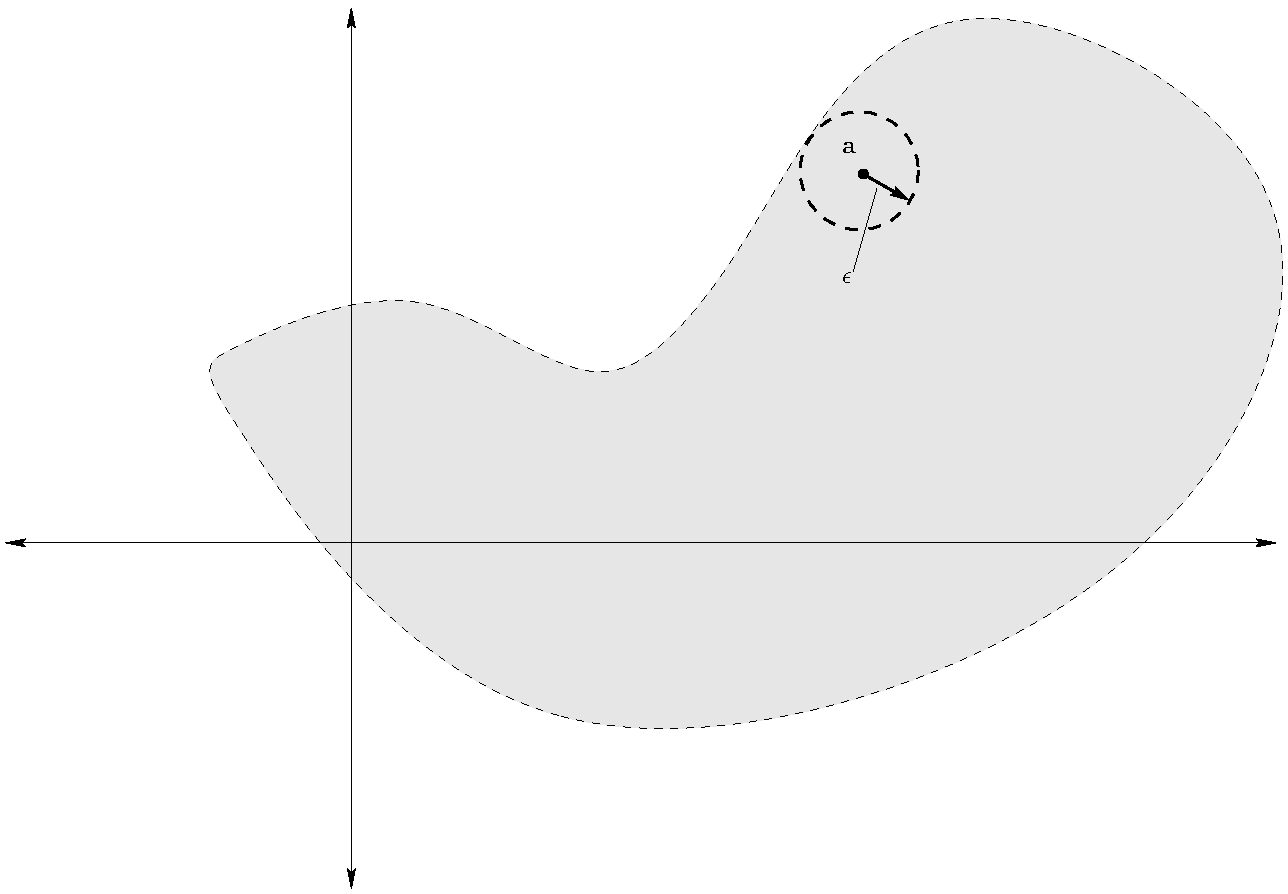
\includegraphics[width=5in]{open.pdf}
\end{center}
You should think of an open set as one where, no matter what point in the set you're at, you've got at least a little bit of room to move, in any direction, without finding yourself outside of the set. In particular, an open set cannot contain its boundary, which we can define precisely as follows:
\begin{definition}
Let $A\subseteq \R^n$ be a given subset. (The set $A$ need not be open in this definition.) We say that a point $\x\in\R^n$ is a {\bf boundary point} of $A$ if every $\epsilon$-neighbourhood of $\x$ contains both points in $A$ and points not in $A$. The union of a set $A$ with the set of boundary points of $A$ is called the {\bf closure} of $A$, and denoted by $\overline{A}$.
\end{definition}
\begin{remark}
We can also talk about {\em closed} sets: a set $A\subseteq\R^n$ is closed if it contains all of its boundary points; that is, if $\overline{A}=A$. Note that in particular the closure of any set is closed. A closed set can also be characterized by the following property: a set $A$ is closed if and only if its complement $\R^n\setminus A$ is open. (The difference $B\setminus A$ of two sets is defined to be the set of all points that belong to $B$ but do not belong to $A$.)
\end{remark}
\subsection{The metric topology on $\R^n$ (optional)}
The following proposition summarizes how the open sets in $\R^n$ interact (and in particular, how a general open set may be built from $\epsilon$-neighbourhoods).  We note that the four properties listed below are indeed the defining properties of a topology, so that we may paraphrase this proposition as saying that the open sets as defined above determine a topology on $\R^n$. In a general course in topology you would probably encounter several different topologies defined on the same set, which can be interesting, since changing the topology changes what your continuous functions are! (This is mainly for your interest - it's not essential to know this or be able follow the proof, as long as you understand the basic idea of an open set.)
\begin{proposition}\label{prop2}
\begin{enumerate}[(i)]
\item $\R^n$ is open.
\item The empty set $\emptyset$ is open.
\item The union of any collection of open sets is open.
\item The intersection of any finite collection of open sets is open.
\end{enumerate}
\end{proposition}
\begin{proof}
The first statement holds trivially, while the second holds vacuously.  For the third, let $A = \bigcup\limits_{\alpha\in I}A_\alpha$ be the union of some collection of open sets, and let $\x\in A$.  Since $\x\in A$, we know that $\x\in A_\alpha$ for some $\alpha\in I$. (The set $I$ here is an {\em index set} - it could be finite, countably infinite, or even uncountable.) Since $A_\alpha$ is open and $\x\in A$, it follows that there is some $\epsilon>0$ such that $N_\epsilon(\x)\subseteq A_\alpha$, and since $A_\alpha\subseteq A$, we obtain (c).  The proof of (d) is left to the reader.
\end{proof}
\section{Limits and continuity}
Let $f:A\subset \R^n\to \R^m$ be a given function with domain $A$ an open subset of $\R^n$. (The domain of a function does not need to be an open set, but it's easiest to define the limit in terms of open sets.) The definition of the limit of $f$ is the natural extension of the single-variable limit, and in fact, it looks almost exactly the same in terms of the vector notation we agreed to stick with above.
\begin{definition}
Let $f:A\subseteq \R^n\to \R^m$ be defined on an open subset $A\subseteq\R^n$, and let $\mathbf{a}$ be any point in the closure $\overline{A}$ of $A$ (i.e. $\mathbf{a}$ is either in the domain of $f$, or on the boundary of the domain). We say that the {\bf limit} of $f$ as $\x$ approaches $\mathbf{a}$ is $\mathbf{b}\in\R^m$, and write
\[
\lim_{\x\to\mathbf{a}}f(\x) = \mathbf{b},
\]
if for every $\epsilon>0$, there is a $\delta>0$ such that if $\x\in A$ and $\x\in N_\delta(\mathbf{a})$, then $f(\x)\in N_\epsilon(\mathbf{b})$.
\end{definition}
(Note that we must have $\x\in A$ so that $f(\x)$ is defined. We can state the two conditions $\x\in A$ and $\x\in N_\epsilon(\mathbf{A})$ more concisely by requiring that $\x$ belong to the intersection $A\cap N_\epsilon(\mathbf{a})$. The definition of the limit often requires that we take $\x$ to lie in the deleted $\epsilon$-neighbourhood $N_\epsilon(\mathbf{a})\setminus\{\mathbf{a}\}$, since $f$ may not be defined at $\mathbf{a}$; however, by intersecting $N_\epsilon(\mathbf{a})$ with the domain $A$, we make sure that $f(\x)$ is defined.)

Written in terms of the distance defined by the vector magnitude, our definition states that given an $\epsilon>0$,  we must be able to find a $\delta>0$ such that whenever $0<\len{\x-\mathbf{a}}<\delta$, we have $\len{f(\x)-\mathbf{b}}<\epsilon$.
\begin{center}
 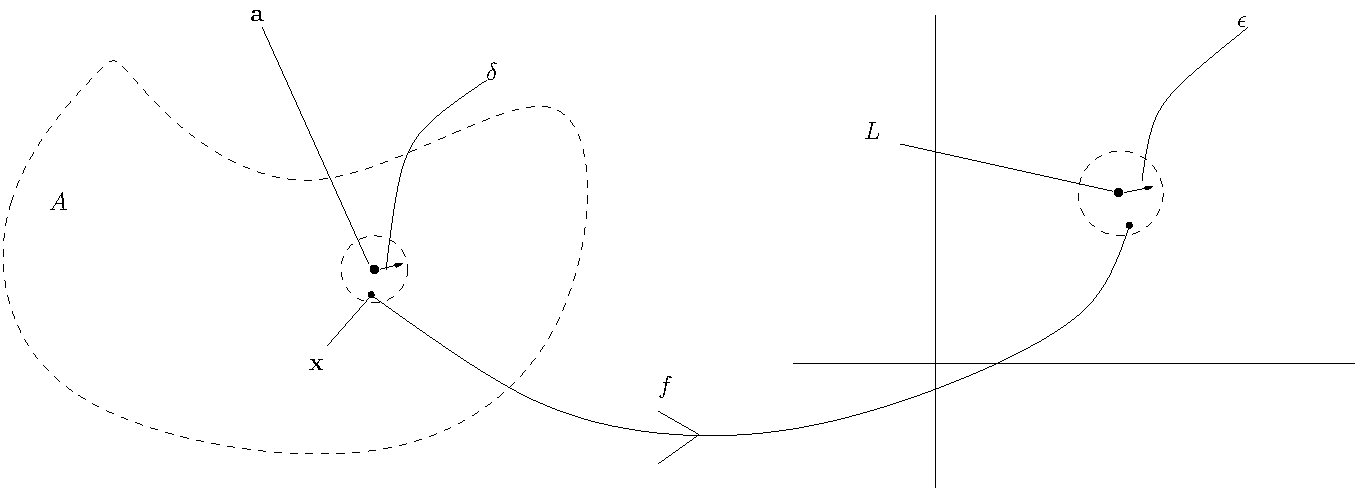
\includegraphics[width=6.5in]{limit.pdf}
\end{center}
Using our definition of the limit (which is a precise definition, incidentally), we can prove all of the usual properties of limits that one is used to having in the calculus of functions of a real variable.
\begin{proposition}
 If $\lim\limits_{\x\to \mathbf{a}} f(\x)$ exists, then it is unique.
\end{proposition}
\begin{proof}
 Suppose that we have $\lim\limits_{\x\to \mathbf{a}} f(\x)=\mathbf{b}_1$ and $\lim\limits_{\x\to \mathbf{a}} f(\x)=\mathbf{b}_2$, where $\mathbf{b}_1\neq \mathbf{b}_2$.  Since $\mathbf{b}_1-\mathbf{b}_2\neq \mathbf{0}$, we have $\len{\mathbf{b}_1-\mathbf{b}_2}>2\epsilon$ for some $\epsilon>0$.  Moreover, there must exist a $\delta>0$ such that $\x\in N_\delta(\mathbf{a})$ implies that $\len{f(\x)-\mathbf{b}_1}<\epsilon$ and $\len{f(\x)-\mathbf{b}_2}<\epsilon$.  (We know there is a $\delta_1$ for $\mathbf{b}_1$ and a $\delta_2$ for $\mathbf{b}_2$, and we can let $\delta$ be the smaller of these two.)  But then we have
\[
 \len{\mathbf{b}_1-\mathbf{b}_2} = \len{(\mathbf{b}_1-f(\x))+(f(z)-\mathbf{b}_2)}\leq \len{f(\x)-\mathbf{b}_1}+\len{f(\x)-\mathbf{b}_2}<\epsilon+\epsilon = 2\epsilon,
\]
which is a contradiction.
\end{proof}
\begin{proposition}
 Let $f$ and $g$ be two functions with common domain $A\subseteq\R^n$ that take values in $\R^m$. Let $\mathbf{a}\in\overline{A}$. If $\lim\limits_{\x\to \mathbf{a}}f(\x)=\mathbf{b}$ and $\lim\limits_{\x\to \mathbf{a}}g(\x) = \mathbf{c}$, then
\begin{enumerate}[(i)]
 \item $\di \lim_{\x\to \mathbf{a}}(f(\x)+g(z)) = \mathbf{b}+\mathbf{c}$.
 \item $\di \lim_{\x\to \mathbf{a}}(tf(\x)) = t\mathbf{b}$, for any $t\in\R$.
 \item If $m=1$, $\di \lim_{\x\to \mathbf{a}}(f(\x)g(\x)) = bc$.
 \item If $m=1$, $\di \lim_{\x\to \mathbf{a}}\left(\frac{f(\x)}{g(\x)}\right) = \frac{b}{c}$, provided $c\neq 0$.
 \item If $f(\x) = (f_1(\x),f_2(\x),\ldots, f_m(\x))$, where the $f_i:A\to \R$, for $i=1,\ldots, m$, are the components of $f$, then
 \[
 \lim_{\x\to\mathbf{a}}f(\x) = \mathbf{b} = \langle b_1,b_2,\ldots, b_m\rangle
 \]
 if and only if
 \[
 \lim_{\x\to\mathbf{a}}f_i(\x) = b_i \text{ for each } i=1,\ldots, m.
 \]
\end{enumerate}
\end{proposition}
We will skip the proofs of these results. If you're interested in seeing the $\epsilon-\delta$ proofs of these limit laws, you may consult, for example, the text by Marsden and Tromba (or any advanced vector calculus text).

Having dealt with limits, we can take care of continuity in the usual way:
\begin{definition}
 Let $A\subseteq \R^n$ be an open set, and let $\x\in A$.  We say that $f:A\to\R^m$ is {\bf continuous} at $\x$ provided
\[
 \lim_{\x\to \mathbf{a}}f(\x) = f(\mathbf{a}),
\]
and that $f$ is continuous {\bf on} $A$ if $f$ is continuous at each $\x\in A$.
\end{definition}
Note that the requirement that $A$ be open allows us to find a $\delta$-neighbourhood of $\x$ contained within $A$, and hence, to evaluate the limit on the left-hand side of the definition.  It follows from the properties of limits that the sum, difference, product and quotient of two continuous functions is continuous.  In addition, the composition of continuous functions is continuous, as you will prove on your fourth assignment.
\begin{remark}
 The definition of continuity {\em on the set} $A$ can be phrased as follows: for any $\epsilon>0$ and for each $\x\in A$, there exists a $\delta>0$ such that if $\len{\x-\y}<\delta$, then $\len{f(\x)-f(\y)}<\epsilon$.  If you wish to be even fancier, see if you can convince yourself that the following definition of continuity is equivalent: $f:A\subseteq R^n\to\R^m$ is continuous if for any open set $U\subseteq\R^m$, the inverse image $f^{-1}(U)\subseteq \R^n$ is open. (The inverse image is the set of all points in $A$ that $f$ sends to $U$.)
\end{remark}



\end{document}